\providecommand{\main}{..}
\documentclass[\main/notes.tex]{subfiles}

\begin{document}
	\setcounter{chapter}{4}
	\chapter{Trigonometry}
		\section{Special Angles}
		\begin{center}
			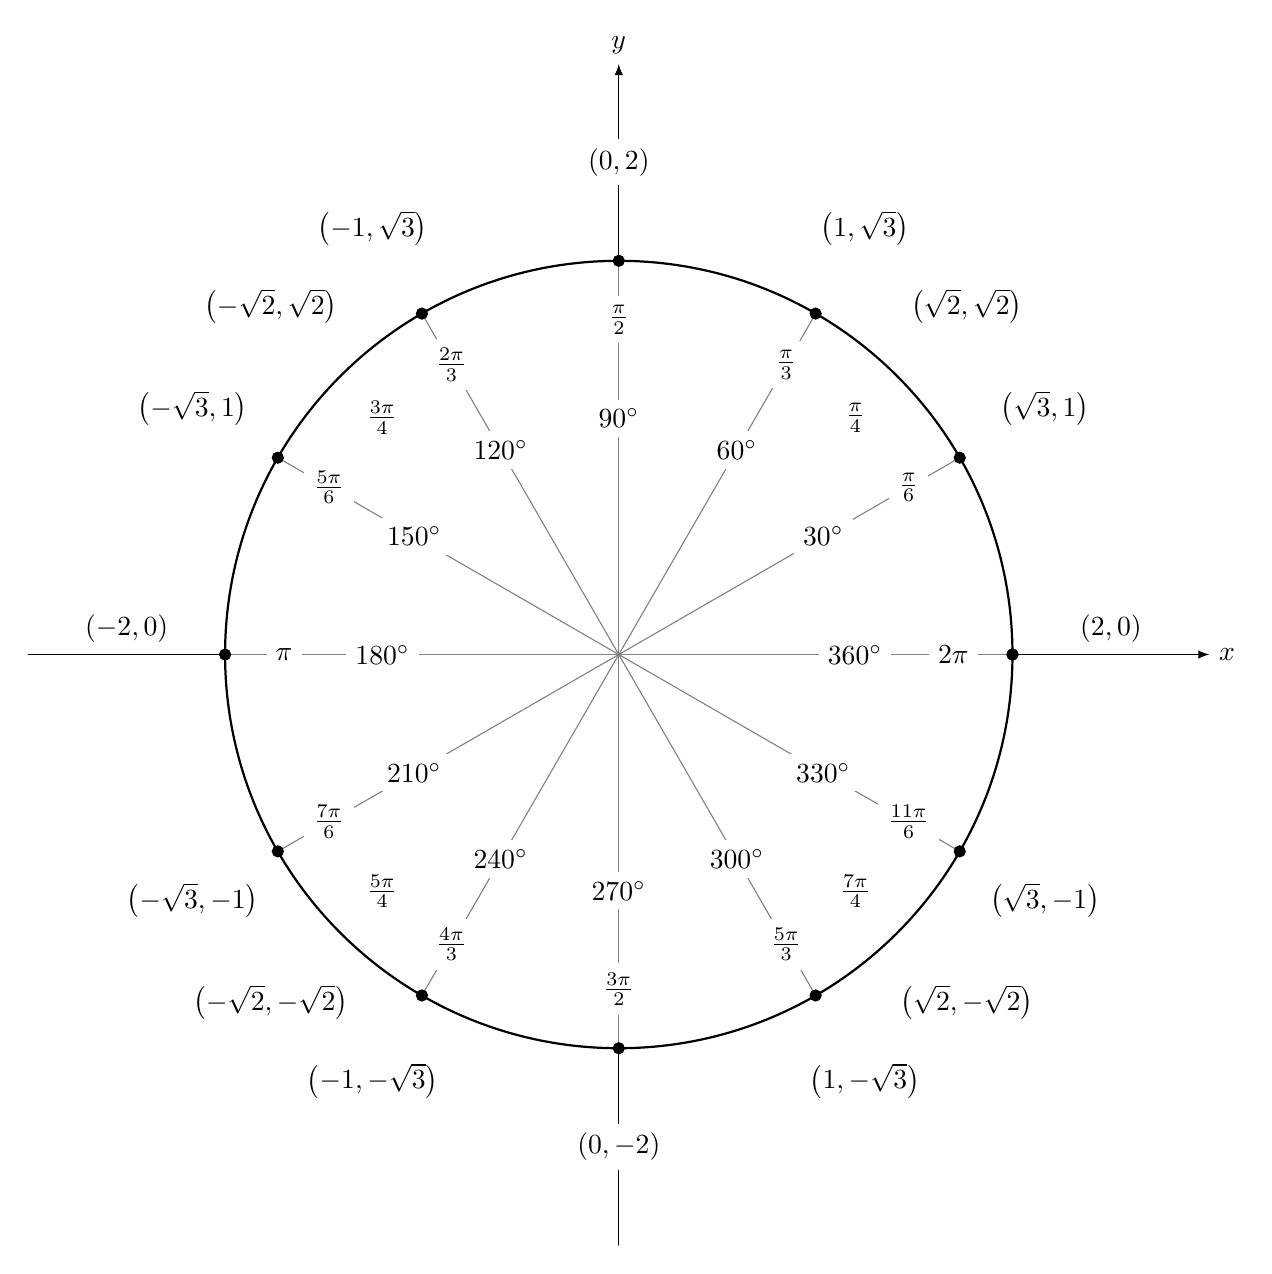
\begin{tikzpicture}[scale=5,cap=round,>=latex]
				% draw the coordinates
				\draw[->] (-1.5cm,0cm) -- (1.5cm,0cm) node[right,fill=white] {$x$};
				\draw[->] (0cm,-1.5cm) -- (0cm,1.5cm) node[above,fill=white] {$y$};

				% draw the unit circle
				\draw[thick] (0cm,0cm) circle(1cm);

				\foreach \x in {0,30,...,360} {
					% lines from center to point
					\draw[gray] (0cm,0cm) -- (\x:1cm);
					% dots at each point
					\filldraw[black] (\x:1cm) circle(0.4pt);
					% draw each angle in degrees
					\draw (\x:0.6cm) node[fill=white] {$\x^\circ$};
				}

				% draw each angle in radians
				\foreach \x/\xtext in {
					30/\frac{\pi}{6},
					45/\frac{\pi}{4},
					60/\frac{\pi}{3},
					90/\frac{\pi}{2},
					120/\frac{2\pi}{3},
					135/\frac{3\pi}{4},
					150/\frac{5\pi}{6},
					180/\pi,
					210/\frac{7\pi}{6},
					225/\frac{5\pi}{4},
					240/\frac{4\pi}{3},
					270/\frac{3\pi}{2},
					300/\frac{5\pi}{3},
					315/\frac{7\pi}{4},
					330/\frac{11\pi}{6},
					360/2\pi}
						\draw (\x:0.85cm) node[fill=white] {$\xtext$};

				\foreach \x/\xtext/\y in {
					% the coordinates for the first quadrant
					30/\sqrt{3}/1,
					45/\sqrt{2}/\sqrt{2},
					60/1/\sqrt{3},
					% the coordinates for the second quadrant
					150/-\sqrt{3}/1,
					135/-\sqrt{2}/\sqrt{2},
					120/-1/\sqrt{3},
					% the coordinates for the third quadrant
					210/-\sqrt{3}/-1,
					225/-\sqrt{2}/-\sqrt{2},
					240/-1/-\sqrt{3},
					% the coordinates for the fourth quadrant
					330/\sqrt{3}/-1,
					315/\sqrt{2}/-\sqrt{2},
					300/1/-\sqrt{3}}
						\draw (\x:1.25cm) node[fill=white] {$\left(\xtext,\y\right)$};

				% draw the horizontal and vertical coordinates
				% the placement is better this way
				\draw (-1.25cm,0cm) node[above=1pt] {$(-2,0)$}
					(1.25cm,0cm)  node[above=1pt] {$(2,0)$}
					(0cm,-1.25cm) node[fill=white] {$(0,-2)$}
					(0cm,1.25cm)  node[fill=white] {$(0,2)$};
			\end{tikzpicture}
		\end{center}
	\section{Identities}
		\subsection{Defining Relations}
			\begin{alignat*}{2}
				\tan \theta &= \frac{\sin\theta}{\cos\theta} \qquad & \cot \theta &= \frac{1}{\tan\theta} = \frac{\cos\theta}{\sin\theta}\\
				\sec\theta &= \frac{1}{\cos\theta} \qquad & \csc\theta &= \frac{1}{\sin\theta}
			\end{alignat*}
		\subsection{Pythagorean Identity}
			\begin{align*}
				\sin^{2}\theta + \cos^{2}\theta = 1
			\end{align*}
		\subsection{Negative Angles}
			\begin{alignat*}{3}
				\sin(-\theta) &= -\sin\theta \qquad & \cos(-\theta) &= \cos\theta \qquad & \tan(-\theta) = -\tan\theta
			\end{alignat*}
		\subsection{Sum and Difference}
			\begin{alignat*}{2}
				\sin(\alpha + \beta) &= \sin\alpha\cos\beta + \cos\alpha\sin\beta \qquad &
				\sin(\alpha - \beta) &= \sin\alpha\cos\beta - \cos\alpha\sin\beta\\
				\cos(\alpha + \beta) &= \cos\alpha\cos\beta - \sin\alpha\sin\beta
			\end{alignat*}
		\subsection{Double Angle Formulae}
			\begin{align*}
				\sin(2\theta) &= 2\sin\theta\cos\theta\\
				\cos(2\theta) &= \cos^{2}\theta - \sin^{2}\theta\\
				&= 2\cos^{2}\theta - 1\\
				&= 1 - 2\sin^{2}\theta
			\end{align*}

	\ifSubfilesClassLoaded{%
		\vbox{\rulechapterend}}{\vspace*{\parskip}\rulebookend}

\end{document}